\documentclass[a4paper,12pt]{article}

% Paquetes
\usepackage[spanish]{babel}
\usepackage[utf8]{inputenc}
\usepackage[T1]{fontenc}
\usepackage{amsmath, amssymb}
\usepackage{graphicx}
\usepackage{siunitx}
\usepackage{subcaption}
\sisetup{output-decimal-marker = {,}}
\usepackage{geometry}
\usepackage{float}

\geometry{margin=2.5cm}

\title{Práctica I: Instrumentación electrónica básica}
\author{Nombre Apellido}
\date{\today}

\begin{document}

\maketitle

\tableofcontents
\newpage


\section{Intrumentación electrónica}

%----------------------------------------
\subsection{Objetivo}

%----------------------------------------
\subsection{Introducción}
La práctica se desarrolló utilizando una placa de pruebas (protoboard) para el montaje de los distintos circuitos eléctricos, garantizando conexiones estables y de baja resistencia entre los componentes. Se empleó un polímetro para la medida de magnitudes eléctricas (resistencia, tensión e intensidad), seleccionando en cada caso la escala adecuada.

En primer lugar, se midieron varias resistencias individuales, comparando los valores experimentales obtenidos con el polímetro con sus valores nominales, con el objetivo de evaluar posibles discrepancias asociadas a tolerancias de fabricación.

Posteriormente, se montaron distintos circuitos resistivos sencillos en la protoboard. Sobre estos montajes se realizaron medidas de tensiones e intensidades en diferentes puntos del circuito, con el fin de comprobar experimentalmente las leyes de Kirchhoff.

A continuación, se construyeron configuraciones específicas para el estudio de los teoremas de Thevenin y Norton. Se determinaron los circuitos equivalentes correspondientes a partir de medidas experimentales, verificando la equivalencia entre ambos modelos.

Finalmente, se analizó el teorema de transferencia máxima de potencia, variando la resistencia de carga y midiendo la potencia disipada en la misma, con el objetivo de identificar la condición de máxima transferencia.

%----------------------------------------
\subsection{Resistencias individuales}


\begin{table}[H]
\centering
\begin{tabular}{cccc}
\hline
Resistencia & Fabricación (k$\Omega$) & Polímetro (k$\Omega$) & Discrepancia (\%) \\
\hline
1 & 0.56 & 0.558 & 0.36 \\
2 & 10 & 10.02 & 0.20 \\
3 & 0.27 & 0.267 & 1.11 \\
4 & 1.6 & 1.606 & 0.38 \\
\hline
\end{tabular}
\caption{Comparación entre valores nominales y medidos de resistencias}
\end{table}


%----------------------------------------
\subsection{Ley de Ohm}

\begin{figure}[h]
    \centering
    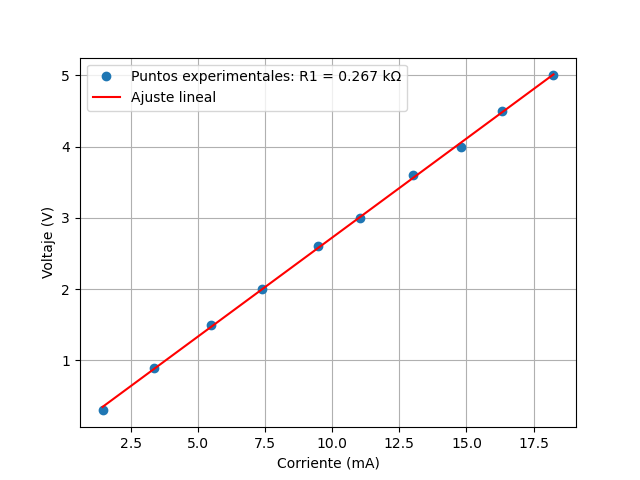
\includegraphics[width=0.8\textwidth]{Figuras/OhmR1.png}
    \caption{Ajuste lineal de la ley de Ohm para la resistencia R1.}
    \label{fig:ohm_R1}
\end{figure}

\begin{table}[h]
    \centering
    \begin{tabular}{|c|c|}
        \hline
        \textbf{Magnitud} & \textbf{Valor} \\
        \hline
        Resistencia nominal (R1) & 0.267 k$\Omega$ \\
        \hline
        Pendiente (R) & $(0.2778 \pm 0.0020)$ k$\Omega$ \\
        \hline
        Ordenada en el origen & $(-0.0538 \pm 0.0014)$ V \\
        \hline
        Coeficiente de determinación ($R^2$) & 0.99957 \\
        \hline
    \end{tabular}
    \caption{Parámetros del ajuste lineal de la ley de Ohm para la resistencia R1.}
    \label{tab:ohm_R1}
\end{table}



\begin{figure}[H]
    \centering
    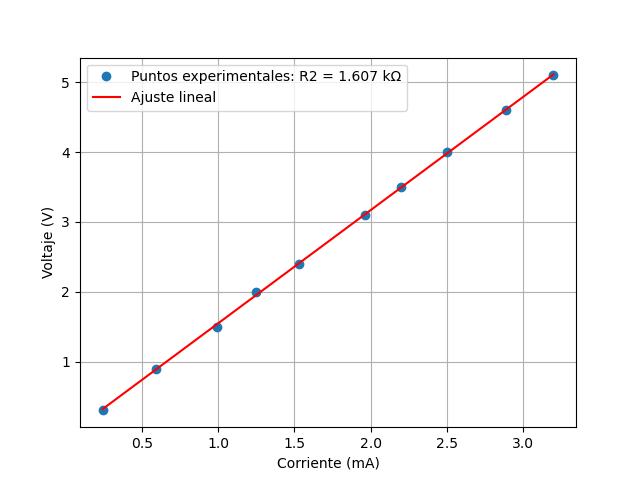
\includegraphics[width=0.8\textwidth]{Figuras/OhmR2.png}
    \caption{Ajuste lineal de la ley de Ohm para la resistencia R2.}
    \label{fig:ohm_R2}
\end{figure}

\begin{table}[H]
    \centering
    \begin{tabular}{|c|c|}
        \hline
        \textbf{Magnitud} & \textbf{Valor} \\
        \hline
        Resistencia nominal (R2) & 1.607 k$\Omega$ \\
        \hline
        Pendiente (R) & $(1.6200 \pm 0.0081)$ k$\Omega$ \\
        \hline
        Ordenada en el origen & $(-0.0706 \pm 0.0054)$ V \\
        \hline
        Coeficiente de determinación ($R^2$) & 0.99980 \\
        \hline
    \end{tabular}
    \caption{Parámetros del ajuste lineal de la ley de Ohm para la resistencia R2.}
    \label{tab:ohm_R2}
\end{table}

\begin{figure}[H]
    \centering
    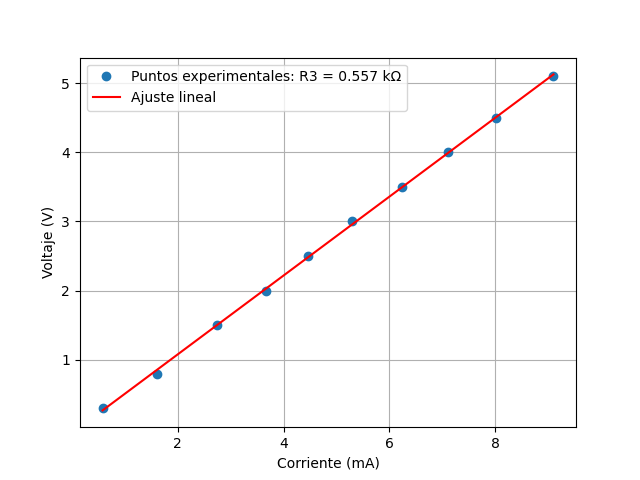
\includegraphics[width=0.8\textwidth]{Figuras/OhmR3.png}
    \caption{Ajuste lineal de la ley de Ohm para la resistencia R3.}
    \label{fig:ohm_R3}
\end{figure}

\begin{table}[H]
    \centering
    \begin{tabular}{|c|c|}
        \hline
        \textbf{Magnitud} & \textbf{Valor} \\
        \hline
        Resistencia nominal (R3) & 0.557 k$\Omega$ \\
        \hline
        Pendiente (R) & $(0.5700 \pm 0.0036)$ k$\Omega$ \\
        \hline
        Ordenada en el origen & $(-0.0617 \pm 0.0024)$ V \\
        \hline
        Coeficiente de determinación ($R^2$) & 0.99968 \\
        \hline
    \end{tabular}
    \caption{Parámetros del ajuste lineal de la ley de Ohm para la resistencia R3.}
    \label{tab:ohm_R3}
\end{table}

\begin{figure}[H]
    \centering
    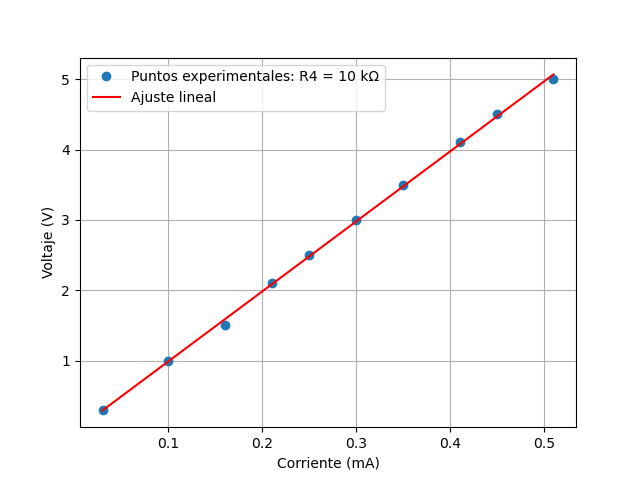
\includegraphics[width=0.8\textwidth]{Figuras/OhmR4.png}
    \caption{Ajuste lineal de la ley de Ohm para la resistencia R4.}
    \label{fig:ohm_R4}
\end{figure}

\begin{table}[H]
    \centering
    \begin{tabular}{|c|c|}
        \hline
        \textbf{Magnitud} & \textbf{Valor} \\
        \hline
        Resistencia nominal (R4) & 10 k$\Omega$ \\
        \hline
        Pendiente (R) & $(9.9470 \pm 0.0937)$ k$\Omega$ \\
        \hline
        Ordenada en el origen & $(-0.0053 \pm 0.0629)$ V \\
        \hline
        Coeficiente de determinación ($R^2$) & 0.99929 \\
        \hline
    \end{tabular}
    \caption{Parámetros del ajuste lineal de la ley de Ohm para la resistencia R4.}
    \label{tab:ohm_R4}
    
    
\begin{table}[H]
\centering
\begin{tabular}{ccc}
\hline
Resistencia & $R \pm \sigma_R$ (k$\Omega$) & $R^2$ \\
\hline
R1 & $0.278 \pm 0.002$ & 0.26700 \\
R2 & $1.620 \pm 0.008$ & 0.99968 \\
R3 & $0.570 \pm 0.004$ & 0.55700 \\
R4 & $9.947 \pm 0.094$ & 0.99929 \\
\hline
\end{tabular}
\caption{Resultados del ajuste lineal V-I}
\end{table} 
    
\end{table}
%----------------------------------------
\subsection{Resistencia en un circuito}

\begin{figure}[H]
    \centering
    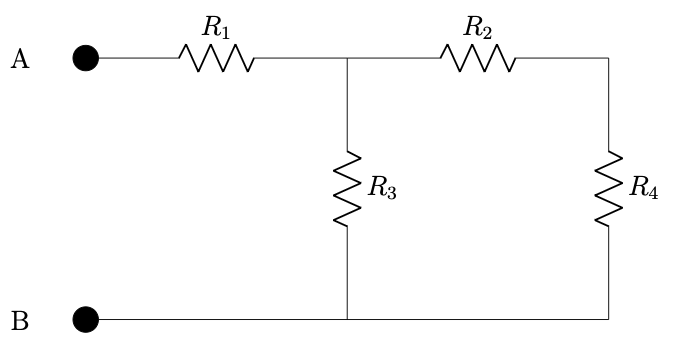
\includegraphics[width=0.8\textwidth]{Figuras/Circuito1.png}
    \caption{Circuito}
    \label{fig:Circuito}
\end{figure}

$R_{\text{eq}} = R_1 + \left( \frac{1}{\frac{1}{R_3} + \frac{1}{R_2 + R_4}} \right)$


\begin{table}[h]
    \centering
    \begin{tabular}{|c|c|}
        \hline
        \textbf{Método} & \textbf{Resistencia equivalente ($\Omega$)} \\
        \hline
        Calculada & $\SI{805.2105}{}$ \\
        \hline
        Medida con polímetro & \SI{805}{} \\
        \hline
    \end{tabular}
    \caption{Comparación entre la resistencia equivalente calculada y la medida experimentalmente.}
    \label{tab:req}
\end{table}

%----------------------------------------
\subsection{Leyes de Kirchhoff}



\begin{table}[h]
    \centering
    \begin{tabular}{|c|c|}
        \hline
        \textbf{Resistencia} & \textbf{Corriente (mA)} $\pm \SI{0.05}{}$ \\
        \hline
        R1 & 6.36 \\
        \hline
        R3 & -6.04 \\
        \hline
        R2 & -0.29 \\
        \hline
    \end{tabular}
    \caption{Corrientes medidas en los nudos del circuito para la verificación de la ley de corrientes de Kirchhoff.}
    \label{tab:kirchhoff_nudos_corriente}
\end{table}



Los resultados obtenidos permiten verificar la ley de corrientes de Kirchhoff. En el nudo analizado, la corriente entrante ($6.36\ \text{mA}$) coincide, dentro del error experimental, con la suma de las corrientes salientes ($6.04 + 0.29 = 6.33\ \text{mA}$). La pequeña discrepancia observada puede atribuirse a las incertidumbres en la medida y a las tolerancias de los componentes, confirmando así la validez de la ley en el circuito estudiado.
\begin{table}[h]
    \centering
    \begin{tabular}{|c|S|S|S|S|}
        \hline
        \textbf{Resistencia} & {R1} & {R2} & {R3} & {R4} \\
        \hline
        {\textbf{Caída de potencial (V)}} & 1.689 & 3.060 & 3.360 & 2.820 \\
        \hline
    \end{tabular}
    \caption{Caídas de potencial medidas en cada resistencia del circuito.}
    \label{tab:kirchhoff_voltajes}
\end{table}

\begin{table}[h]
    \centering
    \begin{tabular}{|c|c|}
        \hline
        \textbf{Malla} & \textbf{Suma de tensiones (V)} \\
        \hline
        Malla 1 $(5 - R_1 - R_3)$ & -0.04900 \\
        \hline
        Malla 2 $(5 - R_1 - R_4 + R_2 - R_3)$ & 0.19100 \\
        \hline
    \end{tabular}
    \caption{Comprobación de la ley de tensiones de Kirchhoff en las mallas del circuito.}
    \label{tab:kirchhoff_mallas}
\end{table}

Los resultados obtenidos permiten verificar la ley de tensiones de Kirchhoff en las mallas del circuito. En ambas mallas, la suma algebraica de las caídas de potencial es próxima a cero, obteniéndose valores de $-0.049\ \text{V}$ y $0.191\ \text{V}$, respectivamente. Estas pequeñas desviaciones respecto al valor teórico nulo pueden atribuirse a errores experimentales, como las incertidumbres en la medida de tensiones y las tolerancias de los componentes. En consecuencia, se confirma que la ley de Kirchhoff se cumple dentro del margen de error experimental.

%----------------------------------------
\subsection{Teoremas de Thévenin y Norton}

Se ha montado el circuito de la Figura~5 con el objetivo de comprobar experimentalmente los teoremas de Thévenin y Norton entre los terminales A y B.

Se realizaron las siguientes medidas:

\begin{itemize}
    \item Tensión en circuito abierto entre A y B, correspondiente a $V_{th}$.
    \item Corriente de cortocircuito entre A y B, correspondiente a $I_N$.
    \item Resistencia equivalente vista desde los terminales, anulando la fuente de tensión (cortocircuitándola).
\end{itemize}


La tensión de Thévenin viene dada por:

\[
V_{th} = \frac{V R_2}{R_1 + R_2}
\]

La resistencia equivalente:

\[
R_{th} = R_3 + R_4 + \frac{R_1 R_2}{R_1 + R_2}
\]

La corriente de Norton se obtiene como:

\[
I_N = \frac{V_{th}}{R_{th}}
\]

\begin{table}[h]
\centering
\begin{tabular}{lccc}
\hline
Magnitud & Teórico & Experimental & Error (\%) \\
\hline
$V_{th}$ (V) & 4.287 & 4.35 & 1.47 \\
$I_N$ (mA) & 0.397 & 0.40 & 0.76 \\
$R_{th}$ (k$\Omega$) & 10.786 & 10.82 & 0.32 \\
\hline
\end{tabular}
\caption{Comparación entre valores teóricos y experimentales}
\end{table}


Los resultados experimentales concuerdan con los valores teóricos dentro de un margen de error inferior al 2\%. Las pequeñas discrepancias se atribuyen a las tolerancias de las resistencias y a las limitaciones de los instrumentos de medida. Se verifica así experimentalmente la validez de los teoremas de Thévenin y Norton.

%----------------------------------------
\subsection{Teorema de transferencia de máxima potencia}

\section{Máxima transferencia de potencia}

Se ha estudiado experimentalmente la potencia disipada en una resistencia de carga conectada entre los terminales A y B del circuito, variando su valor y midiendo la tensión en bornes. A partir de estos datos, se ha calculado la potencia disipada y se ha analizado su dependencia con la resistencia.

La potencia en la carga se ha obtenido mediante:

\[
P = \frac{V^2}{R}
\]

Teóricamente, la potencia transferida es máxima cuando la resistencia de carga coincide con la resistencia de Thévenin del circuito:

\[
R_{\text{carga}} = R_{th}
\]

En este caso, se obtuvo:

\[
R_{th} = 10.82\,\mathrm{k}\Omega
\]

\begin{table}[h]
\centering
\begin{tabular}{lcc}
\hline
Magnitud & Valor & Unidad \\
\hline
Potencia máxima & $4.4 \times 10^{-4}$ & W \\
Resistencia en el máximo & 10040 & $\Omega$ \\
Resistencia izquierda & 7550 & $\Omega$ \\
Resistencia derecha & 12940 & $\Omega$ \\
$R_{th}$ (teórica) & 10820 & $\Omega$ \\
\hline
\end{tabular}
\caption{Resultados experimentales de la potencia en función de la resistencia}
\end{table}

La Figura~\ref{fig:potencia} muestra la dependencia de la potencia con la resistencia de carga.

\begin{table}[h]
\centering
\begin{tabular}{ccc}
\hline
$V$ (V) & $R$ ($\Omega$) & $P$ (W) \\
\hline
\SI{0.448}{} & \SI{1273}{}  & \SI{1.58e-4}{} \\
\SI{1.590}{} & \SI{6350}{}  & \SI{3.98e-4}{} \\
\SI{2.110}{} & \SI{10040}{} & \SI{4.43e-4}{} \\
\SI{2.390}{} & \SI{12940}{} & \SI{4.41e-4}{} \\
\SI{2.630}{} & \SI{16440}{} & \SI{4.21e-4}{} \\
\SI{2.870}{} & \SI{20900}{} & \SI{3.94e-4}{} \\
\SI{3.270}{} & \SI{29700}{} & \SI{3.60e-4}{} \\
\SI{1.797}{} & \SI{7550}{}  & \SI{4.27e-4}{} \\
\hline
\end{tabular}
\caption{Potencia disipada en función de la resistencia de carga}
\end{table}

\begin{figure}[h]
\centering
% Inserta aquí tu figura exportada desde Python
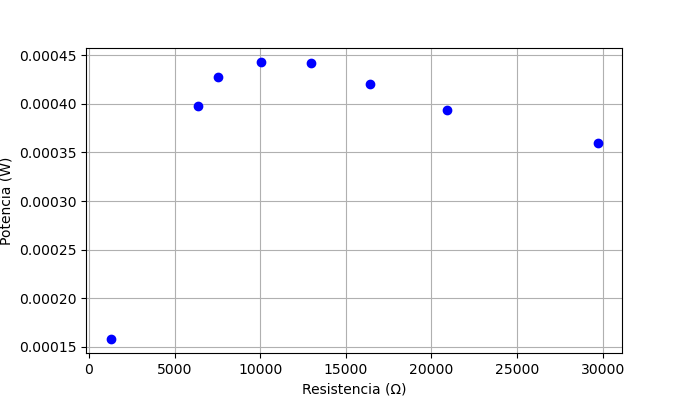
\includegraphics[width=0.7\textwidth]{Figuras/Potencia.png}
\caption{Potencia disipada en función de la resistencia de carga}
\label{fig:potencia}
\end{figure}

Se observa que la potencia presenta un máximo para un valor de resistencia cercano a $R_{th}$. El valor teórico $R_{th}=10820\,\Omega$ se encuentra dentro del intervalo definido por las resistencias adyacentes al máximo experimental ($7550\,\Omega$ y $12940\,\Omega$), lo que confirma el teorema de máxima transferencia de potencia. Las discrepancias se deben a la discretización de los valores de resistencia y a las incertidumbres experimentales.

\section{El Diodo}
\subsection{Introducción y objetivos}

El objetivo de esta práctica es estudiar el comportamiento del diodo semiconductor, analizando su curva característica corriente–tensión y comprendiendo su funcionamiento tanto en polarización directa como inversa. El diodo es un elemento fundamental en la electrónica, especialmente en aplicaciones de conversión de energía como fuentes de alimentación y circuitos de rectificación. Teóricamente, el modelo de Shockley describe la relación corriente–tensión de un diodo real a temperatura constante.

\subsection{Ecuación del diodo}

El comportamiento ideal del diodo en la región activa puede describirse mediante la ecuación exponencial
\begin{equation}
I_d = I_s \left(e^{\frac{q V_d}{\eta k T}} - 1\right),
\end{equation}
donde \(I_s\) es la corriente de saturación, \(q\) la carga elemental, \(k\) la constante de Boltzmann, \(T\) la temperatura absoluta y \(\eta\) el factor de idealidad. En polarización directa (\(V_d>0\)), la corriente aumenta exponencialmente con la tensión y puede aproximarse por
\begin{equation}
I_d \simeq I_s e^{\frac{q V_d}{\eta k T}},
\end{equation}
mientras que en polarización inversa (\(V_d<0\)), la corriente es aproximadamente constante e igual a \(-I_s\).

A continuación se muestran los datos experimentales obtenidos en polarización directa. La columna de \(V_{\text{diodo}}\) se ha corregido para reflejar el signo físico correcto:

\begin{table}[h]
\centering
\begin{tabular}{S S S S}
\hline
{$V_{\text{aplicada}}$ [V]} & {$V_{\text{resistencia}}$ [mV]} & {$V_{\text{diodo}}$ [V]} & {$I_{\text{diodo}}$ [A]} \\
\hline
0   & 0     & 0,0052 & 0 \\
0,3 & 0,01  & 0,314  & 0,00001 \\
0,6 & 0,148 & 0,501  & 0,000148 \\
0,9 & 0,372 & 0,545  & 0,000372 \\
1,2 & 0,64  & 0,572  & 0,00064 \\
1,5 & 0,973 & 0,59   & 0,000973 \\
1,8 & 1,29  & 0,6    & 0,00129 \\
2   & 1,47  & 0,61   & 0,00147 \\
3   & 2,39  & 0,631  & 0,00239 \\
4   & 3,42  & 0,65   & 0,00342 \\
5   & 4,41  & 0,662  & 0,00441 \\
6   & 5,44  & 0,673  & 0,00544 \\
7   & 6,43  & 0,68   & 0,00643 \\
8   & 7,36  & 0,685  & 0,00736 \\
\hline
\end{tabular}
\caption{Medidas experimentales del diodo en polarización directa.}
\label{tab:diodo_directa}
\end{table}

La Figura~\ref{fig:iv_directa} muestra la curva \(I\)–\(V\) para la región directa, junto con el ajuste al modelo teórico. Para visualizar la dependencia exponencial, se realizó también un ajuste lineal de \(\ln(I_d)\) frente a \(V_d\) (Figura~\ref{fig:log_iv_directa}). Los parámetros obtenidos del ajuste se resumen en la Tabla~\ref{tab:ajuste_diodo}. A partir de la pendiente se dedujo el factor de idealidad \(\eta = 2,12 \pm 0,07\), coherente con un diodo de silicio en condiciones experimentales.

\begin{figure}[h]
\centering
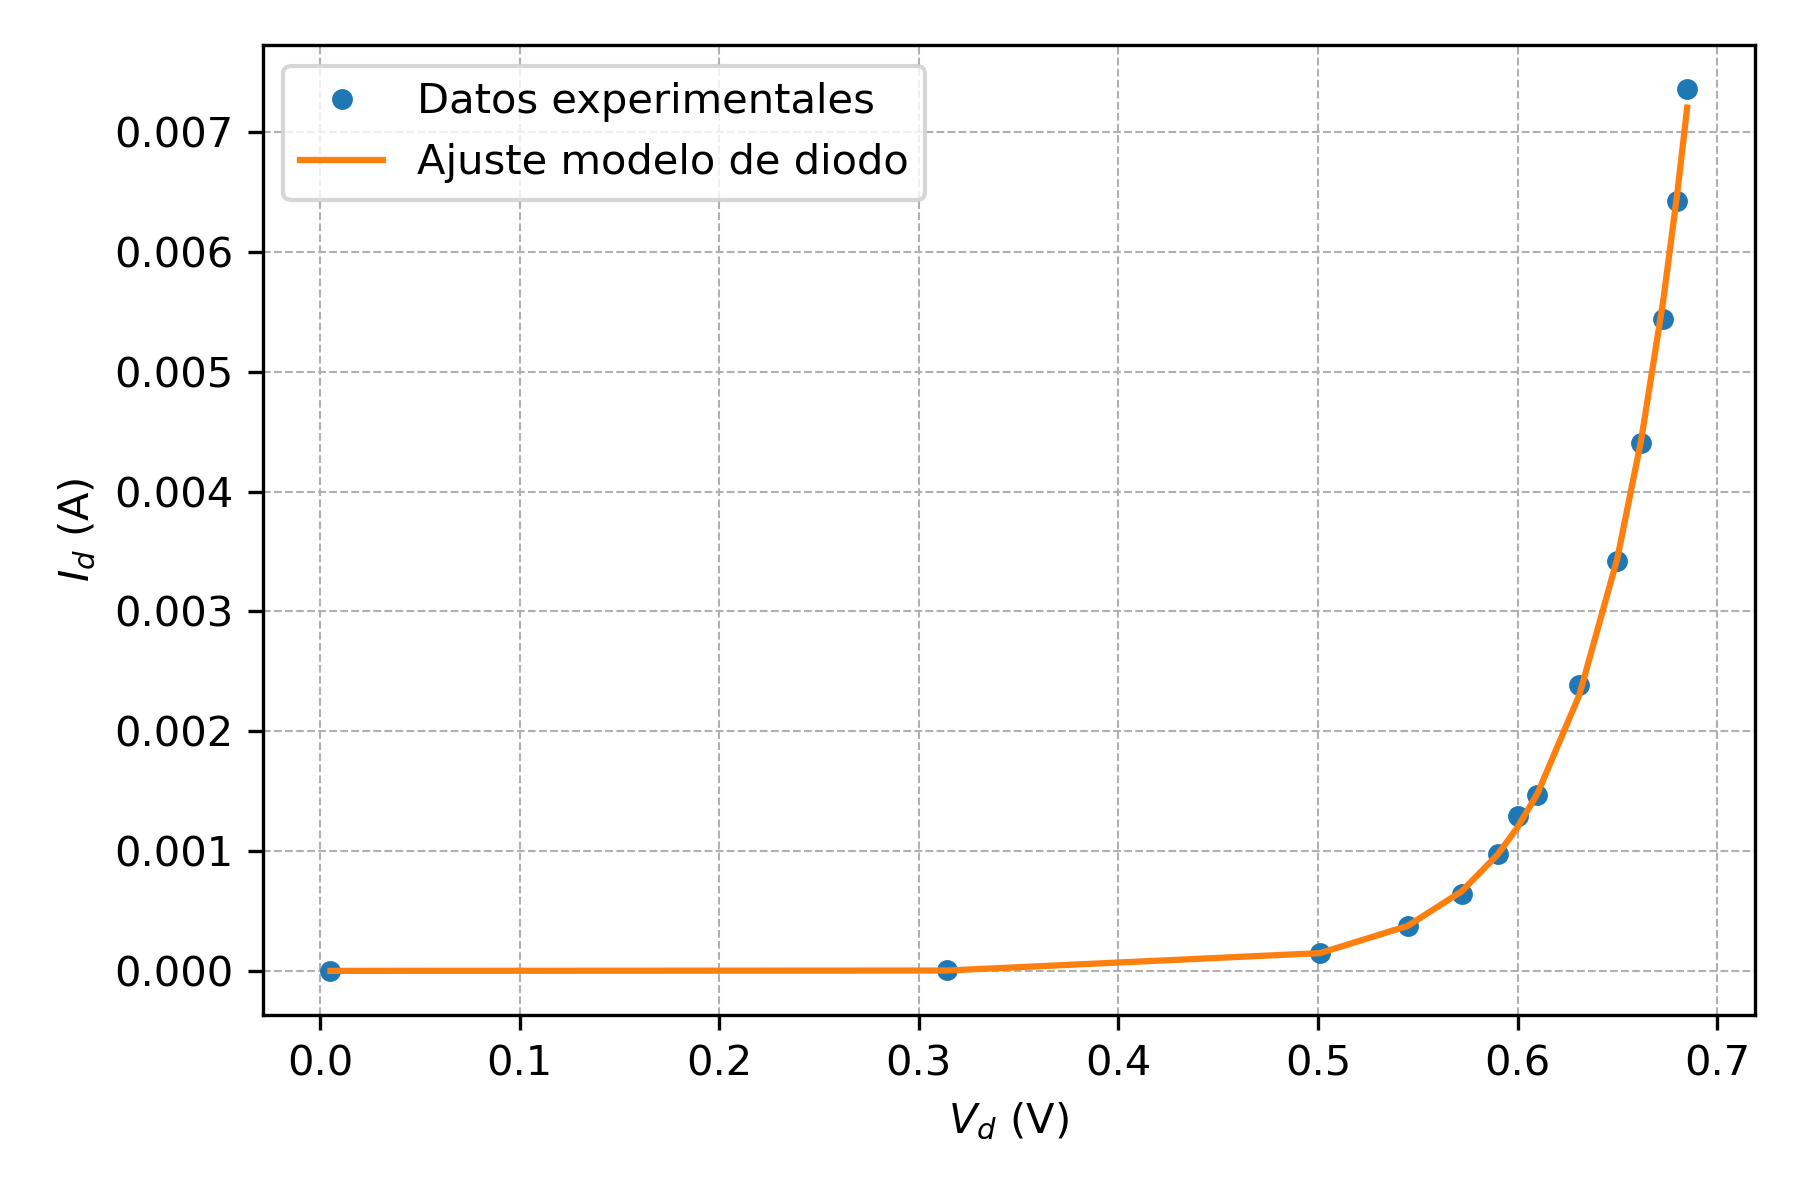
\includegraphics[width=0.7\textwidth]{Figuras/iv_directa.png}
\caption{Curva corriente–tensión del diodo en polarización directa junto con el ajuste al modelo teórico.}
\label{fig:iv_directa}
\end{figure}

\begin{figure}[h]
\centering
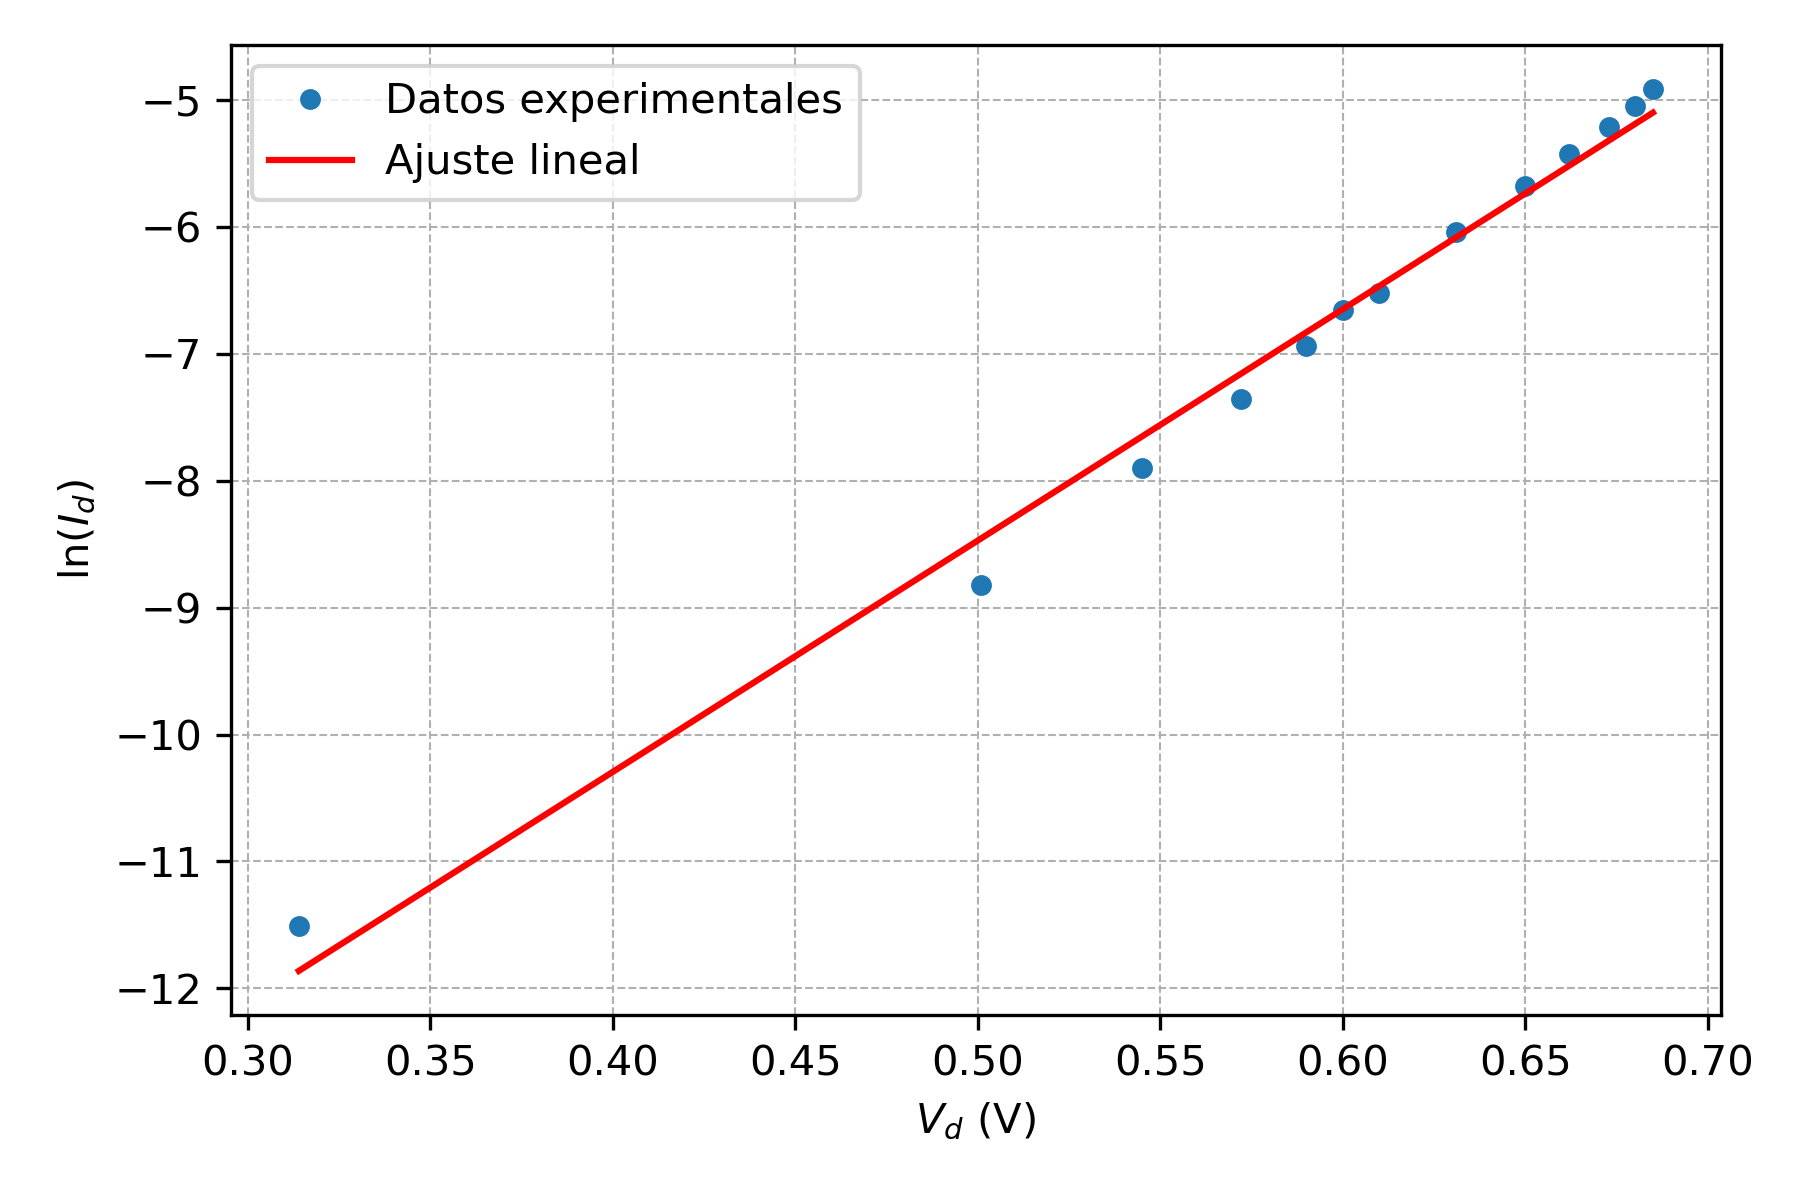
\includegraphics[width=0.7\textwidth]{Figuras/log_iv_directa.png}
\caption{Representación de $\ln(I_d)$ frente a $V_d$ en polarización directa y ajuste lineal.}
\label{fig:log_iv_directa}
\end{figure}

\begin{table}[H]
\centering
\begin{tabular}{lc}
\hline
Parámetro & Valor \\
\hline
Pendiente $a$ (\si{\volt^{-1}}) & $18,24 \pm 0,58$ \\
Ordenada $b=\ln(I_s)$            & $-17,59 \pm 1,00$ \\
Coeficiente de determinación $R^2$ & $0,989$ \\
\hline
\end{tabular}
\caption{Parámetros obtenidos del ajuste lineal de $\ln(I_d)$ frente a $V_d$.}
\label{tab:ajuste_diodo}
\end{table}

Para polarización inversa no se detectó caída de tensión apreciable en la resistencia, lo que implica una corriente menor que el umbral de medida. Los valores de $V_d$ registrados y la corriente deducida se presentan en la Tabla~\ref{tab:diodo_inversa} y la Figura~\ref{fig:iv_inversa}. La curva completa $I$–$V$ del diodo, mostrando ambas regiones, se presenta en la Figura~\ref{fig:iv_total}.

\begin{table}[H]
\centering
\begin{tabular}{S S S S}
\hline
{$V_{\text{aplicada}}$ [V]} & {$V_{\text{resistencia}}$ [mV]} & {$V_{\text{diodo}}$ [V]} & {$I_{\text{diodo}}$ [A]} \\
\hline
0    & 0 & -0,02  & 0 \\
-0,5 & 0 & -0,516 & 0 \\
-1   & 0 & -1,101 & 0 \\
-1,5 & 0 & -1,571 & 0 \\
-2   & 0 & -2,13  & 0 \\
-3   & 0 & -3,03  & 0 \\
-4   & 0 & -4,1   & 0 \\
-5   & 0 & -5,04  & 0 \\
-6   & 0 & -6,09  & 0 \\
-7   & 0 & -7,05  & 0 \\
-8   & 0 & -8,09  & 0 \\
\hline
\end{tabular}
\caption{Medidas experimentales del diodo en polarización inversa.}
\label{tab:diodo_inversa}
\end{table}

\begin{figure}[H]
\centering
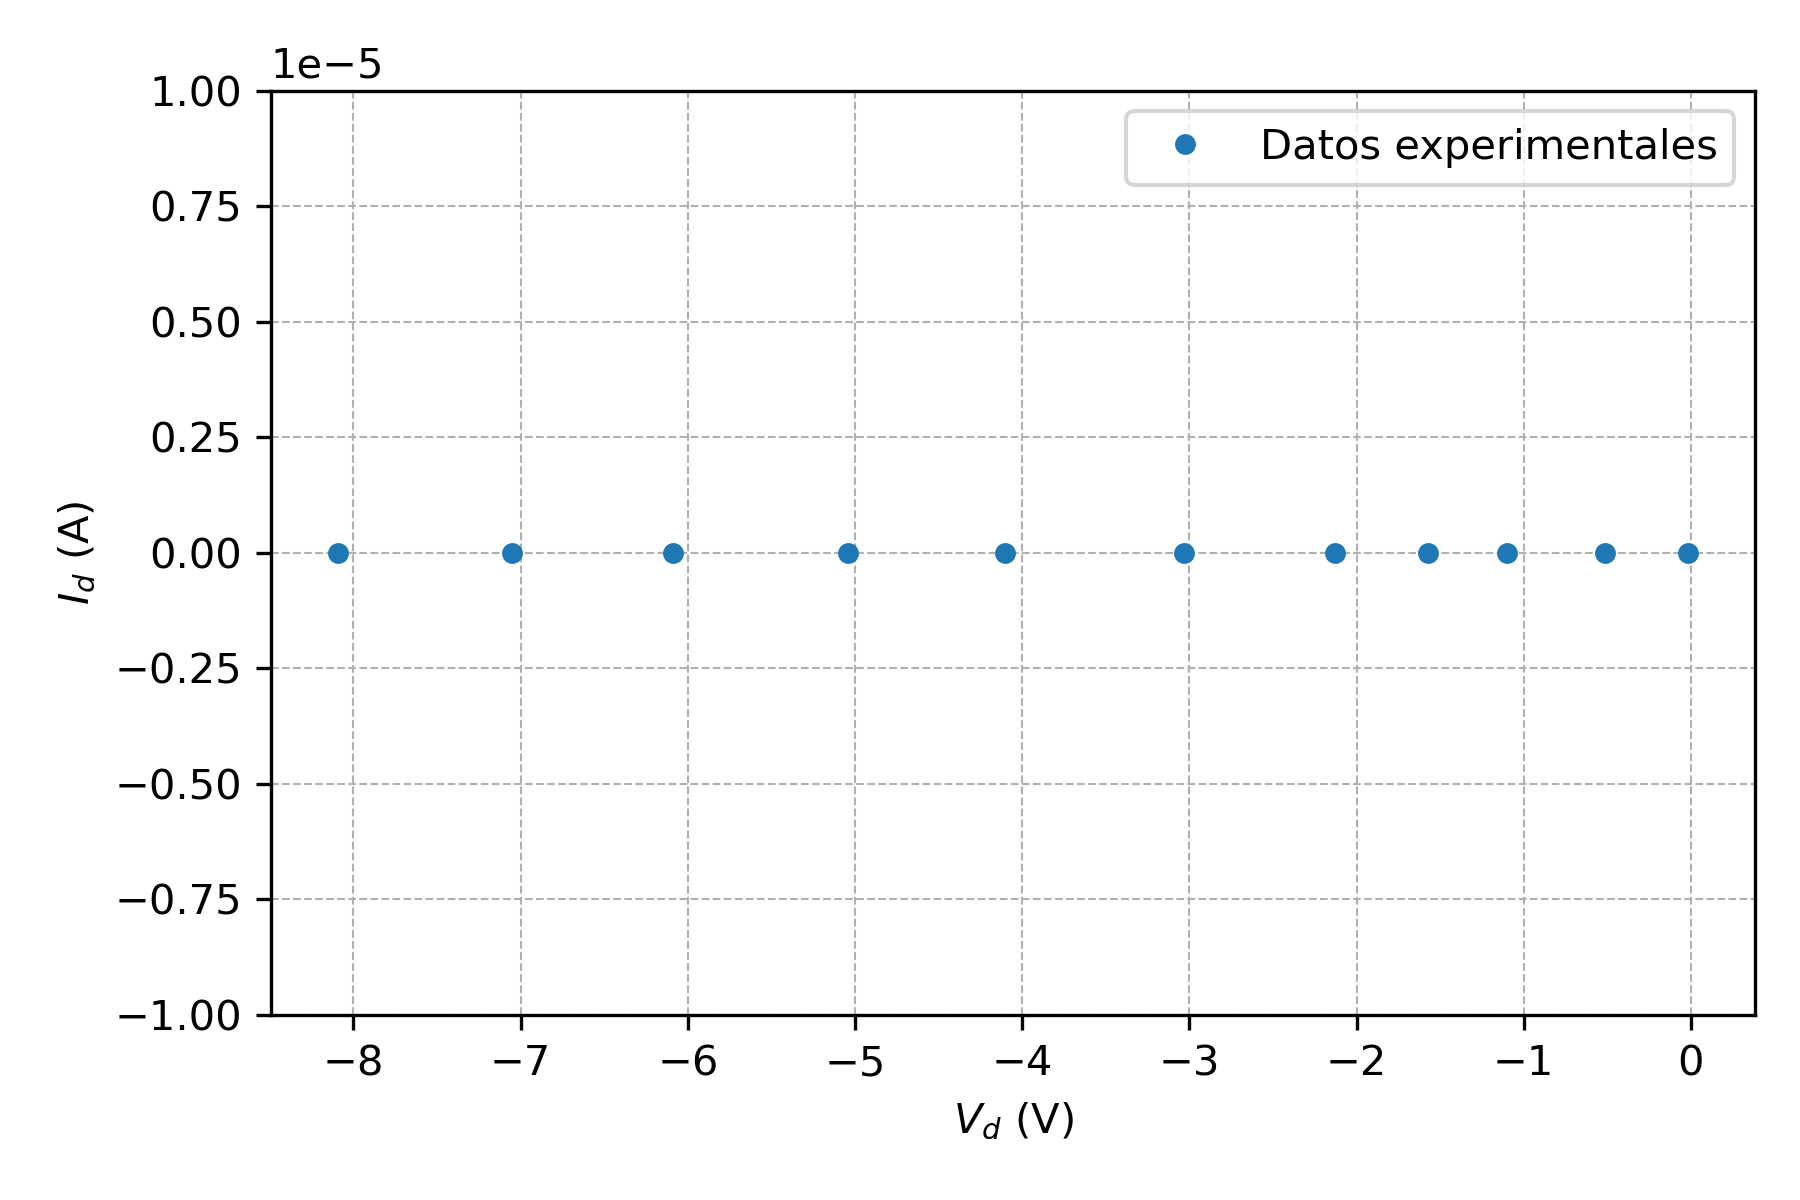
\includegraphics[width=0.7\textwidth]{Figuras/iv_inversa.png}
\caption{Curva corriente–tensión del diodo en polarización inversa. La corriente medida es nula dentro de la resolución experimental.}
\label{fig:iv_inversa}
\end{figure}

\begin{figure}[H]
\centering
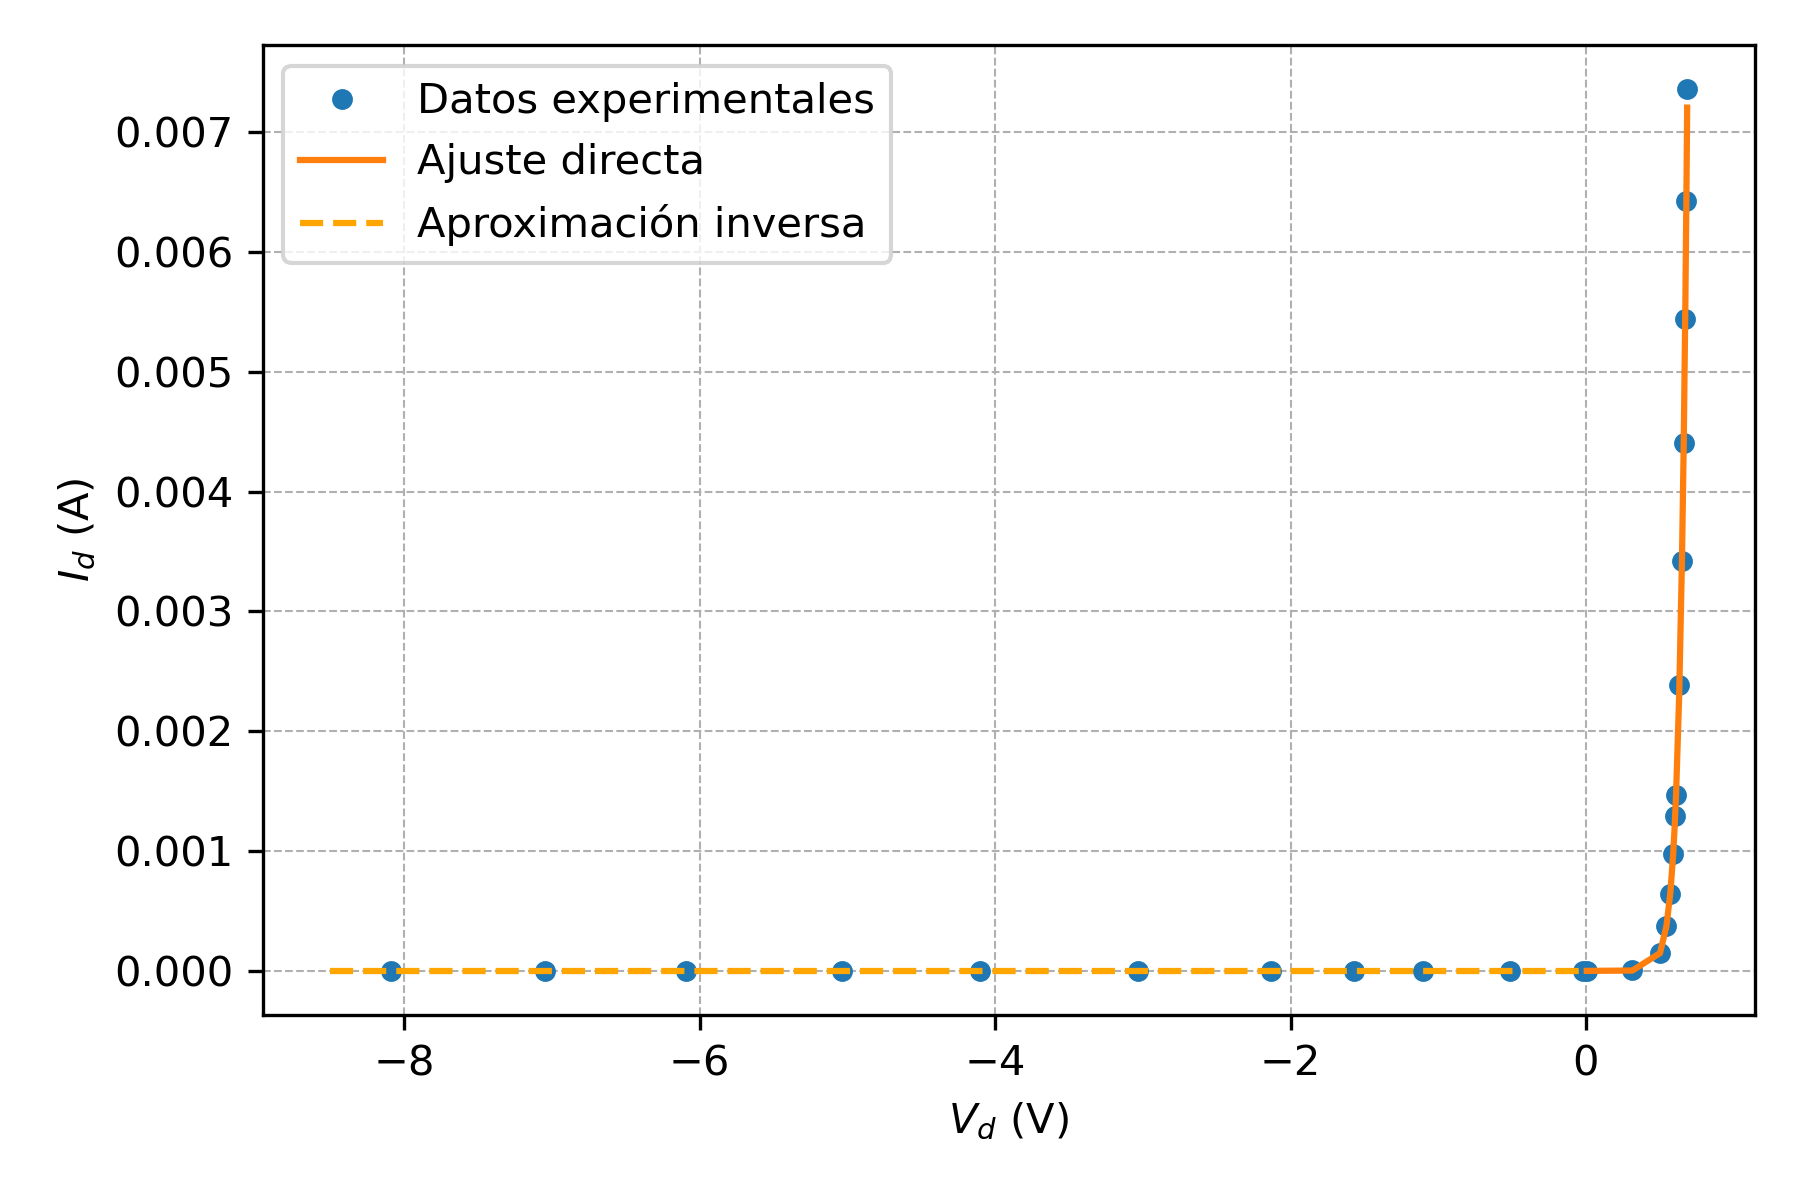
\includegraphics[width=0.7\textwidth]{Figuras/iv_total.png}
\caption{Curva completa $I$–$V$ del diodo, mostrando las regiones de polarización directa e inversa junto con los ajustes teóricos correspondientes.}
\label{fig:iv_total}
\end{figure}

\subsection{Fuente de alimentación}

En esta etapa se estudia la conversión de una señal alterna en una señal unidireccional mediante rectificación. Se han empleado dos configuraciones: el rectificador de media onda y el rectificador de onda completa.

\subsubsection{Rectificador de media onda}

La Figura~\ref{fig:rectificador_media_onda} muestra el circuito de media onda utilizado, formado por un diodo y una carga resistiva. El diodo conduce durante los semiciclos positivos de la tensión de entrada y bloquea los negativos, de modo que la señal de salida es un tren de pulsos positivos. La señal observada en el osciloscopio se recoge en la Figura~\ref{fig:senal_media_onda}.

\begin{figure}[H]
\centering
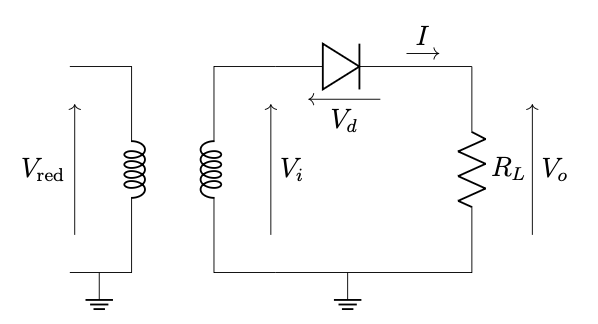
\includegraphics[width=0.7\textwidth]{Figuras/MediaOnda.png}
\caption{Esquema del rectificador de media onda utilizado en la práctica.}
\label{fig:rectificador_media_onda}
\end{figure}

\begin{figure}[H]
\centering
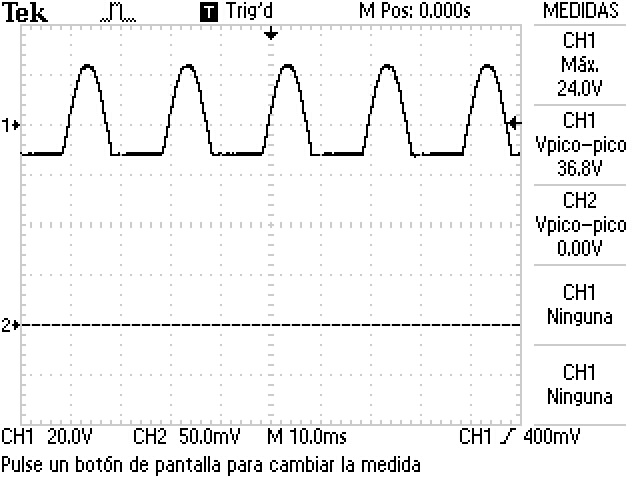
\includegraphics[width=0.7\textwidth]{Figuras/Rect_media.jpeg}
\caption{Señal de salida del rectificador de media onda observada en el osciloscopio. Se aprecia cómo el diodo permite el paso de los semiciclos positivos, bloqueando los negativos.}
\label{fig:senal_media_onda}
\end{figure}

\subsubsection{Rectificador de onda completa}

Para mejorar la eficiencia se emplea un puente de diodos que rectifica ambos semiciclos de la señal de entrada, duplicando la frecuencia de la salida y reduciendo el rizado. El esquema del puente se muestra en la Figura~\ref{fig:rectificador_onda_completa}, y la señal de salida medida se presenta en la Figura~\ref{fig:senal_onda_completa}. En comparación con la media onda, el rectificador de onda completa aprovecha toda la señal de entrada y proporciona una tensión media mayor.

\begin{figure}[H]
\centering
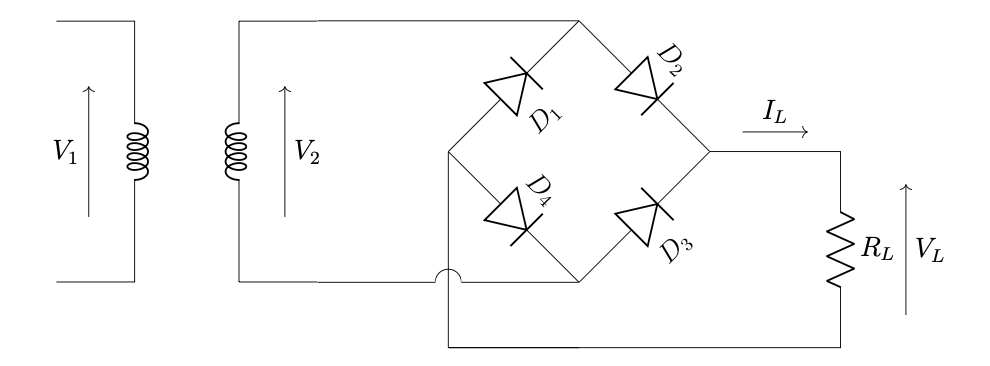
\includegraphics[width=0.7\textwidth]{Figuras/OndaCompleta.png}
\caption{Esquema del rectificador de onda completa mediante puente de diodos.}
\label{fig:rectificador_onda_completa}
\end{figure}

\begin{figure}[H]
\centering
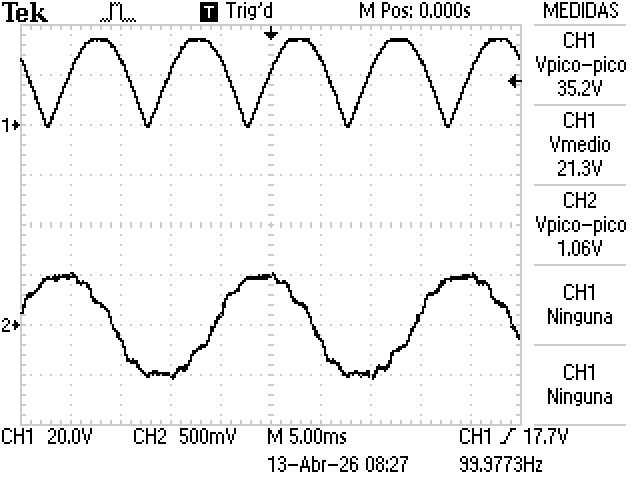
\includegraphics[width=0.7\textwidth]{Figuras/Rect_completa.jpeg}
\caption{Señales de entrada (abajo) y salida (arriba) del rectificador de onda completa observadas en el osciloscopio. La salida presenta únicamente valores positivos correspondientes a la rectificación de ambos semiciclos.}
\label{fig:senal_onda_completa}
\end{figure}

\subsection{Filtrado}

Tras la rectificación, la salida presenta una componente de continua superpuesta a un rizado significativo. Para reducirlo se incorpora un condensador en paralelo con la carga. La Figura~\ref{fig:filtrado_comparacion} recoge las señales de salida para capacidades de \SI{47}{\micro\farad} y \SI{100}{\micro\farad}. La Tabla~\ref{tab:filtrado} resume el valor medio y la amplitud de rizado. Se observa que al incrementar la capacidad disminuye el rizado y aumenta ligeramente la tensión media, puesto que el condensador se descarga más lentamente entre semiciclos.

\begin{figure}[h]
\centering
\begin{subfigure}{0.48\textwidth}
    \centering
    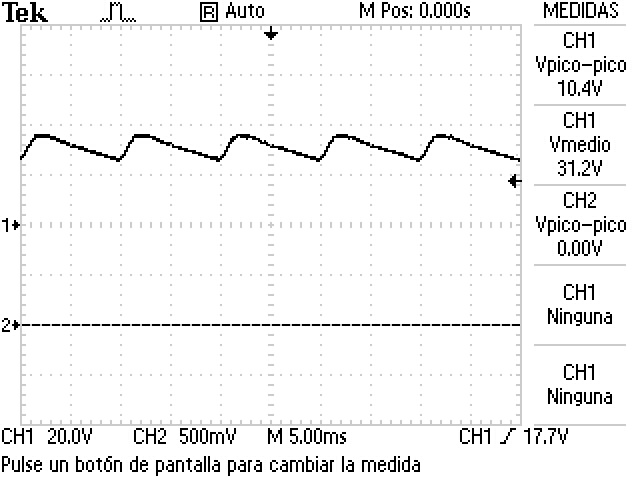
\includegraphics[width=\textwidth]{Figuras/Filtado47.jpeg}
    \caption{$C = \SI{47}{\micro\farad}$}
    \label{fig:filtrado_47}
\end{subfigure}
\hfill
\begin{subfigure}{0.48\textwidth}
    \centering
    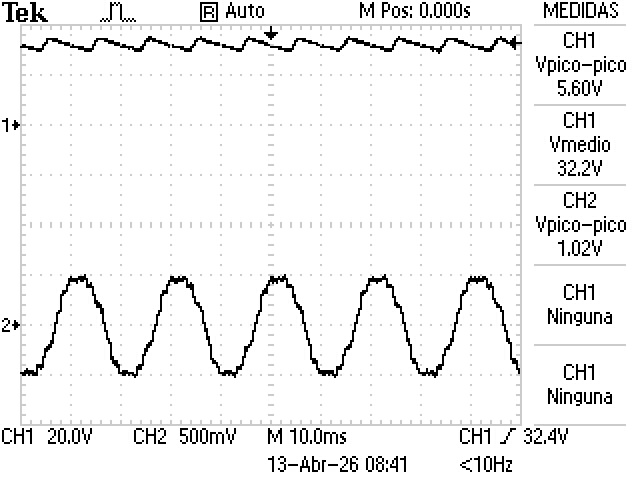
\includegraphics[width=\textwidth]{Figuras/Fitrado100.jpeg}
    \caption{$C = \SI{100}{\micro\farad}$}
    \label{fig:filtrado_100}
\end{subfigure}
\caption{Señales de salida del rectificador con filtrado capacitivo para dos valores de capacidad. Se aprecia cómo la amplitud del rizado disminuye al aumentar $C$.}
\label{fig:filtrado_comparacion}
\end{figure}

\begin{table}[h]
\centering
\begin{tabular}{ccc}
\hline
$C$ (\si{\micro\farad}) & $V_{\text{pp}}$ (V) & $V_{\text{med}}$ (V) \\
\hline
47  & 10,4 & 31,1 \\
100 & 5,6  & 32,2 \\
\hline
\end{tabular}
\caption{Valores de tensión pico a pico (rizado) y tensión media para distintos condensadores de filtrado.}
\label{tab:filtrado}
\end{table}

El rizado disminuye aproximadamente de \SI{10,4}{\volt} a \SI{5,6}{\volt} al pasar de \SI{47}{\micro\farad} a \SI{100}{\micro\farad}, mientras que la tensión media aumenta de \SI{31,1}{\volt} a \SI{32,2}{\volt}. Estos resultados evidencian que aumentar la capacidad del condensador mejora el filtrado y aproxima la señal de salida a una tensión continua.

\subsection{Regulador de tensión}

El filtrado capacitivo reduce el rizado, pero la tensión de salida aún depende de la carga y de la tensión de entrada. Para obtener una tensión continua estable se emplea un regulador LM317. Su circuito se muestra en la Figura~\ref{fig:regulador}, donde la tensión de salida viene determinada por
\begin{equation}
V_{\text{out}} = 1{,}25 \left(1 + \frac{R_2}{R_1}\right).
\end{equation}
Fijando $R_1=\SI{267}{\ohm}$ y deseando \SI{5}{\volt} a la salida, se obtiene $R_2 \approx \SI{801}{\ohm}$. En el montaje se utilizó $R_2=\SI{800}{\ohm}$, obteniéndose un valor próximo al deseado.

\begin{figure}[H]
\centering
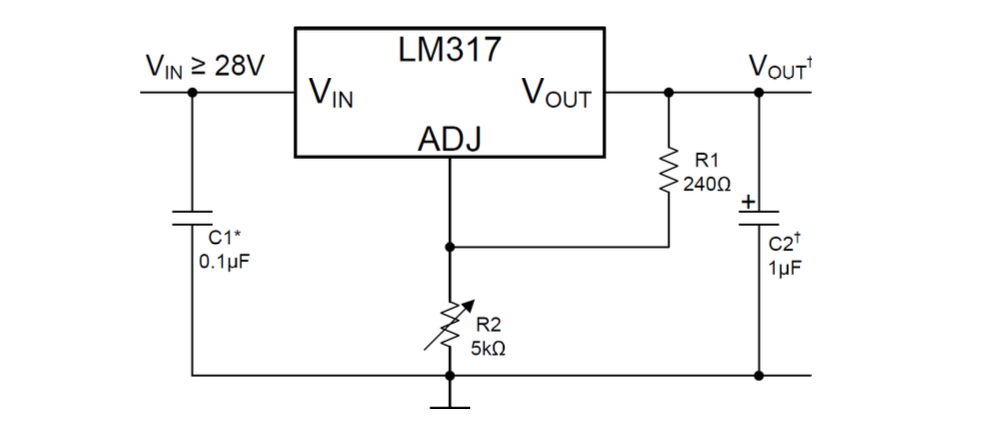
\includegraphics[width=0.6\textwidth]{Figuras/Regulador.png}
\caption{Esquema del regulador de tensión basado en el circuito integrado LM317.}
\label{fig:regulador}
\end{figure}

La salida del regulador se recogió mediante una fotografía del osciloscopio (Figura~\ref{fig:regulador_salida}). La traza superior corresponde a la tensión regulada y aparece prácticamente como una línea recta. La tensión media es \SI{4,73}{\volt} y la amplitud del rizado residual es de aproximadamente \SI{600}{\milli\volt}, valor mucho menor que el observado con filtrado únicamente. Ello confirma el correcto funcionamiento del regulador, que proporciona una salida continua prácticamente independiente de la carga y de las variaciones de entrada.

\begin{figure}[h]
\centering
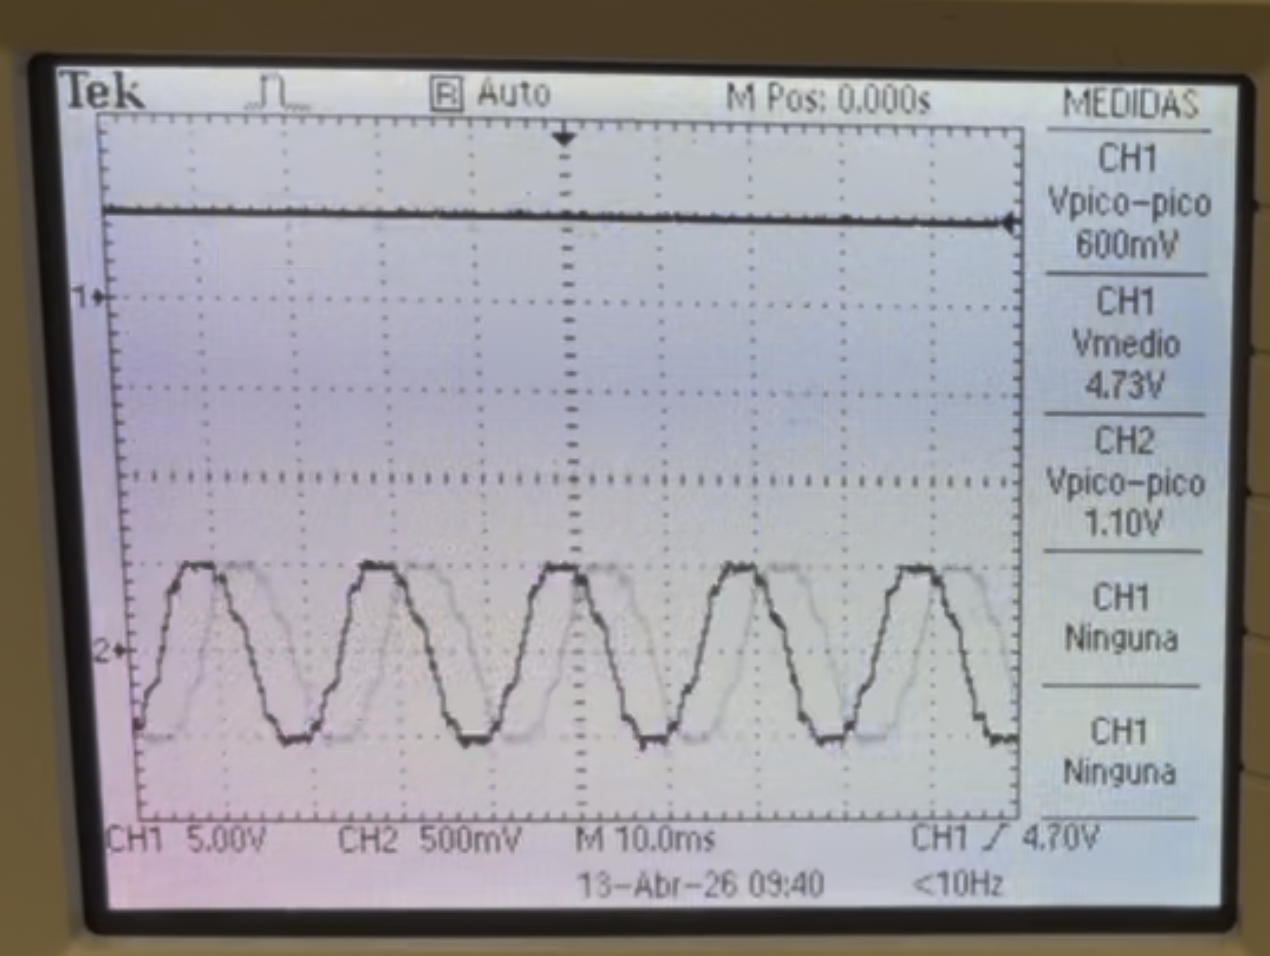
\includegraphics[width=0.6\textwidth]{Figuras/Regulador_osciloscopio.jpeg}
\caption{Señal de salida del regulador LM317 obtenida mediante captura fotográfica del osciloscopio. La traza superior corresponde a la salida regulada, con rizado reducido ($V_{pp} \approx \SI{600}{\milli\volt}$) y valor medio de \SI{4,73}{\volt}.}
\label{fig:regulador_salida}
\end{figure}
%----------------------------------------%----------------------------------------
\subsection{Cuestiones}

%----------------------------------------
\begin{thebibliography}{9}

\bibitem{ref1}
Referencia aquí

\end{thebibliography}

\end{document}